\section[Měření neutronů aktivační metodou]{Stanovení neutronových polí, účinných průřezů a štěpných výtěžků využitím aktivační techniky}

Většina důležitých informací je v otázkách 9-11.

\subsection{Aktivační měření s dozimetrickými foliemi}

Měření probíhá tak, že vložíme aktivační detektor (folie o známé tloušťce, hmotnosti a materiálu) do neutronového pole a poté za pomoci spektrometrie určíme reakční rychlost:

\begin{equation}
    \boxed{R = \int_{E_{min}}^{E_{max}} \phi(E) \sigma(E) \: \text{d}E = \dfrac{S \lambda \dfrac{t_\text{real}}{t_\text{live}}}{N_0 \: \varepsilon \: I \: (1-e^{-\lambda t_a}) \: e^{-\lambda t_v} \: (1-e^{-\lambda t_\text{real}}),}}
\end{equation}

případně produkční rychlost (furt ty samé vztahy):

\begin{equation}
    \boxed{P =  \dfrac{S \lambda \dfrac{t_\text{real}}{t_\text{live}}}{\varepsilon \: I \: (1-e^{-\lambda t_a}) \: e^{-\lambda t_v} \: (1-e^{-\lambda t_\text{real}}).}}
\end{equation}

Tato měření pak pomohou pomoct v dalších odvětvích (teď mimo NAA, té se věnuje předešlá otázka).

\subsubsection{Měření účinných průřezů}

Hojně využívané pro měření účinných průřezů prahových reakcí (na urychlovači). Jako zdroj neutonů se použije svazek protonů, které odstřelují tenkou Li folii (p + Li), což produkuje proud kvazimonoenergetických neutronů, které jsou dobře odlišitelné od pozadí. Dále možné využít beryliový terčík (p + Be).

\begin{figure}[H]
    \centering
    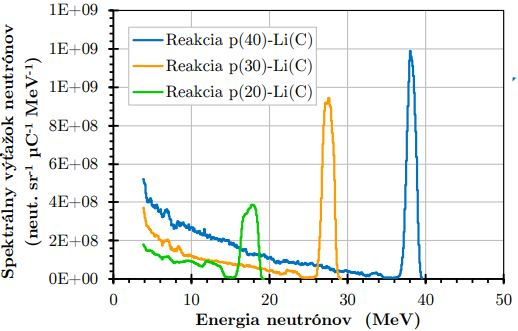
\includegraphics[width=0.5\textwidth]{img/p+Li_E.JPG}
    \caption{Neutronové spektrum pro reakci (p + Li).}
\end{figure}

Tím, jak měním rychlost primárních protonů jsem schopný sekundární neutronový peak posouvat do různých energiích. Tyto sekundární neutrony poté ozařují zkoumaný materiál, jehož účinný průřez měřím. Takto změřím někoik bodů (dle energie), které poté vyhodnocuji a dle čehož stanovím závislost $\sigma$ na $E$. Tato metoda se využívá v ÚJF AV ČR v Řeži.

\subsubsection{Spektrometrie neutronových polí}

Spektrometrii neutronů je věnována celá předchozí otázka, tahle kapitolka je pouze o smektrometrii aktivační technikou. Ve zkoumaném neutronovém poli se ozáří několik odlišných aktivačních detektorů: Cd, Mo, Y, Cu, In, Co apod., přičemž materiály se vybírají podle toho, jak jsou citlivé v jiných oblastech energie neutronů.

Po ozáření opět proběhne gamma spektrometrie a u každé folie se stanoví sada reakčních rychlostí. Jelikož známe průběhy účinných průřezů na těchto materiálech, je pak možné zpětně zrekonstruovat neutronové spektrum. K tomu se využívají různé kódy, my pracovali s kódem SAND-II (podobně jako v případě měření Bonnerovými sférami).

\begin{figure}[H]
    \centering
    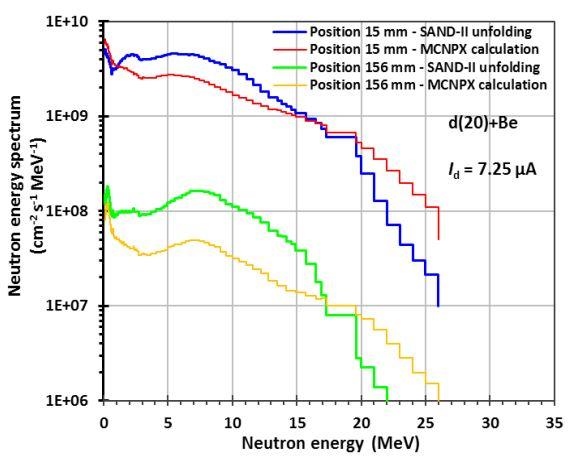
\includegraphics[width=0.5\textwidth]{img/spektrum_aktivacne.JPG}
    \caption{Zpětná rekompozice neutronového spektra pro reakci (d + Be).}
\end{figure}

\subsubsection{Stanovení štěpných výtěžků}

Nic jsme si o tom neříkali, ale předpokládám, že ozářím folii ze štěpného materiálu v neutronovém poli a poté změřím reakční rychlost pro štěpné produkty, které se zde vyprodukovali. Na tomto základě pak asi bude možné zpětně určit výtěžky pro konkrétní štěpný produkt.

DOPLNIT??